%!TEX root = main.tex
\subsection{Описание работы программы}

Запуск программы осуществляется через исполняемый файл \texttt{DEFcodes.app} в операционной системе Mac OS X, \texttt{DEFcodes.exe} в ОС Windows. Этот исполняемый файл запускает среду выполнения node-webkit, которая выполняет первоначальную настройку согласно файлу \texttt{package.json}\footnote{Файл \texttt{package.json} един для различных ОС} (Листинг \ref{lst:packagejson}).

\lstcode{codes/package.json}{0.6}{\small}{package.json}{packagejson}

Точкой входа в программу является файл \texttt{index.html} (Листинг~\ref{lst:indexhtml}). Базовый шаблон, в который входит основная верстка интерфейса: контейнеры, заголовки, и~т.~п.,  инициализируется с помощью Javascript-функции \texttt{initBaseTemplate()} (Листинг~\ref{lst:initbasetemplate}).

\begin{figure}[H]
	\centering
	\begin{subfigure}[r]{0.45\textwidth}
		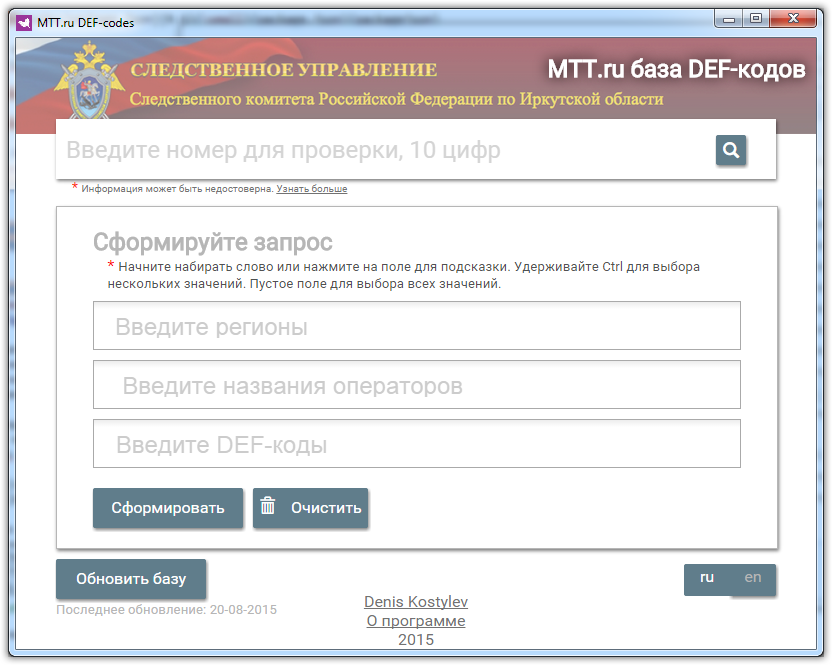
\includegraphics[width=\textwidth]{pics/screens/win_main.png}
		\caption{Windows 7}
	\end{subfigure}
	\quad
	\begin{subfigure}[l]{0.45\textwidth}
		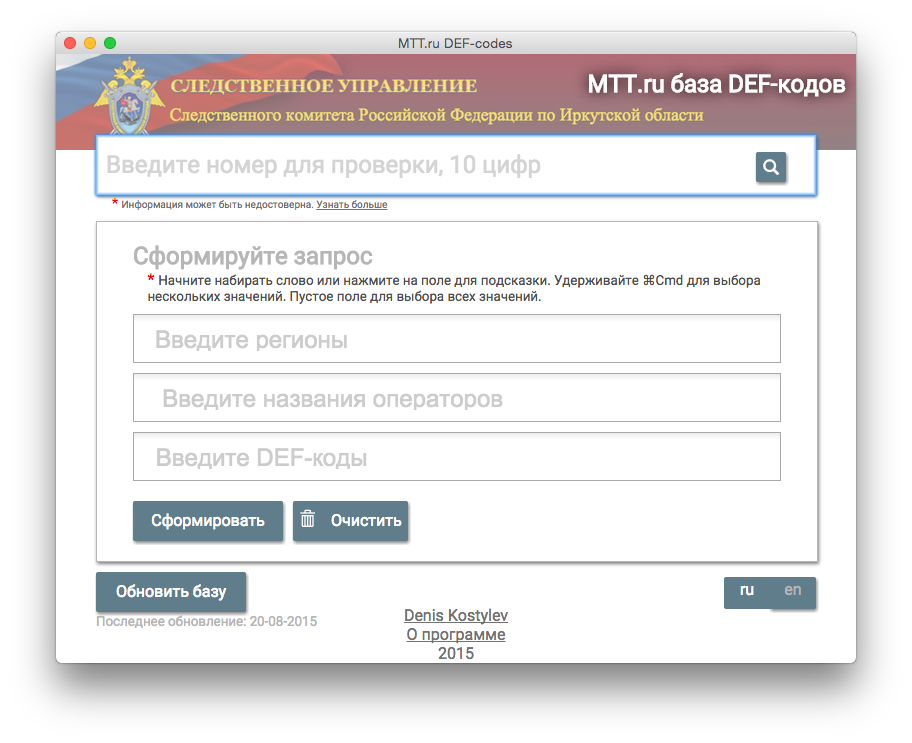
\includegraphics[width=\textwidth]{pics/screens/mac_main.png}
		\caption{Mac OS X 10.10}
	\end{subfigure}
	\caption{Окно программы при запуске программы}
	\label{fig:mainscreen}
\end{figure}

\begin{leftbar}
	На рисунке~\ref{fig:mainscreen} дизайн программы был спроектирован в соответствии с концепцией Material Design\cite{materialdesign}.
	
	Были использованы иконки из набора Twitter Bootstrap и FontAwesome. Иконка приложения --- логотип сайта \url{http://mtt.ru}.
\end{leftbar}

\lstcode{codes/index.html}{0.6}{\small}{index.html}{indexhtml}

\lstcode{codes/initBaseTemplate().js}{0.6}{\small}{initBaseTemplate}{initbasetemplate}

\begin{leftbar}
	В данной программе реализована мультиязычность, это значит, что все используемые в программе тексты загружаются из внешних файлов. В настоящий момент используются два языка: русский (основной, загружается при запуске) и английский. Языковые файлы находятся в каталоге ./lang --- ru.json и en.json для русского и английского языка соответственно. Файл русского языка приведен ниже (Листинг~\ref{lst:rujson})	
\end{leftbar}

\lstcode{codes/ru.json}{0.3}{\footnotesize}{Файл перевода}{rujson}

После инициализации базового шаблона, программа формирует расширенный шаблон --- добавляет надписи, кнопки и другие элементы управления, а также присваивает их событиям определенные функции. После чего начинается инициализация базы (Листинг~\ref{lst:baseinit}), данные из JSON-файла преобразовываются в объекты и загружаются в оперативную память.

Также в этом методе осуществляется проверка даты обновления базы. При отсутствии обновлений базы в течение месяца, программа выводит соответствующее уведомление.

\lstcode{codes/base_init().js}{0.6}{\small}{base\_init()}{baseinit}

Затем формируется список автодополнения и инициализируется плагин командой \texttt{<selector>.chosen()}.

\lstcode{codes/initAutocomplete().js}{0.6}{\small}{initAutocomplete}{initautocomplete}

Для реализации фильтрации вывода сначала был использован стандартный элемент HTML для ввода текстовой информации --- \texttt{<input>} с подключенным расширением jQueryUI autocomplete\cite{jqueryui-autocomplete}. Однако, руководитель от предприятия внес соответствующие пожелания к использованию данного интерфейса. Выбранный модуль не позволял выбирать несколько значений из списка, не открывая его заново для каждого значения.

Впоследствии этот элемент был заменен на стандартный HTML-элемент \texttt{<select>}, с подключенной библиотекой chosen\cite{chosen}. Данный модуль решил вышеуказанную проблему --- для выбора нескольких значений достаточно удерживать клавишу-модификатор (Ctrl для ОС Windows и Cmd для Mac OS).

\begin{figure}[H]
	\centering
	\begin{subfigure}[r]{0.45\textwidth}
		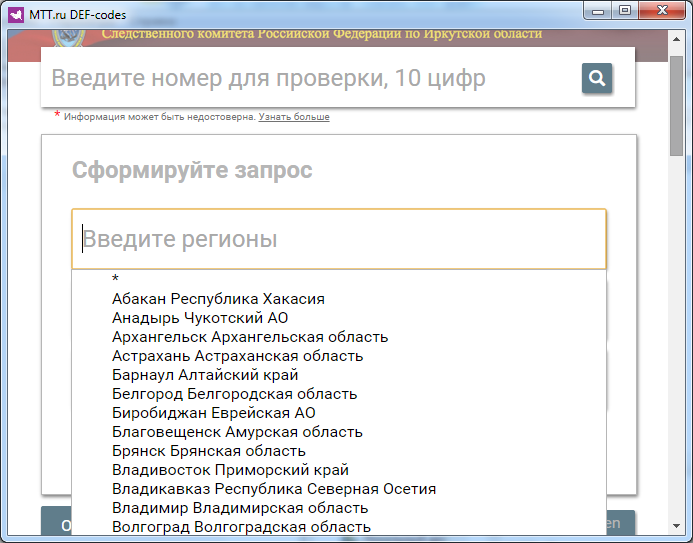
\includegraphics[width=\textwidth]{pics/screens/win_autocomp.png}
		\caption{Windows 7}
	\end{subfigure}
	\quad
	\begin{subfigure}[l]{0.45\textwidth}
		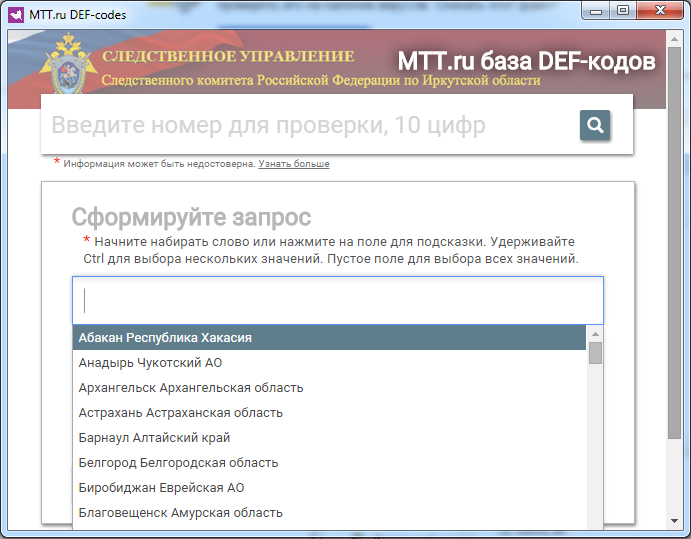
\includegraphics[width=\textwidth]{pics/screens/win_chosen.png}
		\caption{Mac OS X 10.10}
	\end{subfigure}
	\caption{Сравнение модулей для фильтрации данных на примере выбора области в ОС Windows}
\end{figure}

Также в приложении предусмотрен режим отладки. Если переменная \texttt{logging} равна \texttt{True}, то в каталоге ./logs создается текстовый файл с именем даты и время запуска программы, в который записывается информация о работе приложения: свойства компьютера, на котором запущена программа; и ход работы приложения (пример файла журнала приведен ниже). При этом в стандартный поток вывода (в фреймворке node-webkit также встроена Javascript консоль, но она скрыта от пользователя в финальной версии программы) отправляются данные о длительности выполнения той или иной функции.

\begin{framed}
	\noindent
	27-08-2015-16-59-57: Application is launched \\
	27-08-2015-16-59-57: OS Platform: win32 \\
	27-08-2015-16-59-57: OS Type: Windows\_NT \\
	27-08-2015-16-59-57: OS Release: 6.1.7601 \\
	27-08-2015-16-59-57: OS Arch: ia32 \\
	27-08-2015-16-59-57: OS Hostname: Denis-PC \\
	27-08-2015-16-59-57: Begin initialization \\
	27-08-2015-16-59-57: Chosen language file is ru \\
	27-08-2015-16-59-57: Extended template is initialized \\
	27-08-2015-16-59-57: Staring initialization of base \\
	27-08-2015-16-59-57: Begin parsing lang-JSON \\
	27-08-2015-16-59-57: Basic template is initialized \\
	27-08-2015-16-59-57: Starting initialization of basic template \\
	27-08-2015-16-59-57: starting initialization of extended template \\
	27-08-2015-16-59-57: base is opened \\
	27-08-2015-16-59-57: locations is formed \\
	27-08-2015-17-01-10: Export modal is opened \\
	27-08-2015-17-01-18: Starting export to txt  \\
	27-08-2015-17-01-18: Folder 27-08-2015-17-01-18 is created  \\
	27-08-2015-17-01-20: Starting export to excel  \\
	27-08-2015-17-01-20: Excel file is created  \\
	27-08-2015-17-01-20: Sheet Абакан  Республика Хакасия is created  \\
	27-08-2015-17-01-20: Sheet Анадырь  Чукотский АО is created \\
	<...>
\end{framed}

Все файлы исходных кодов были минимизированы и к каждому был создан .map-файл, что ускорило работу программы.

%!TEX root = main.tex
\subsubsection{Загрузка базы DEF-кодов}

Для загрузки базы с удаленного адреса была создана программа на языке программирования Python (Листинг~\ref{lst:dwnldData}).

В процессе анализа работы сервиса был выявлен формат запроса для получения базы с url \url{http://mtt.ru/defcodes}. Он имеет следующий вид (Листинг~\ref{lst:request})

\lstcode{codes/request.py}{0.6}{\small}{Формат запроса}{request}

Отправление запроса происходит методом \texttt{post}, который содержится в модуле \texttt{requests}. Данный оператор принимает два аргумента: адрес и параметры запроса, указанные выше.

Ответ от сервера приходит в формате JSON, который содержит два поля:
\begin{enumerate*}
	\item \texttt{'status'} --- состояние ответа (success --- данные успешно получены; error --- возникла ошибка; captcha --- слишком много запросов с IP-адреса и неверно указан проверочный код);
	\item \texttt{'resultHTML'} --- база DEF-кодов в формате HTML-таблицы.
\end{enumerate*}
 
После получения успешного ответа от сервера, программа сохраняет локальную копию в файл \texttt{base.html} и начинает анализ таблицы. Для данной операции используется модуль BeautifulSoup, которая позволяет работать с сущностями таблицы как с объектами. Проанализированные данные программа сохраняет в JSON-файл \texttt{base.json}, с которым в последствии работает основное приложение.

\lstcode{codes/dwnldData.py}{0.6}{\small}{Python-скрипт для загрузки базы DEF-кодов}{dwnldData}

Готовый скрипт упакован с помощью утилит "py2app" для Mac OS X и "py2exe" для Windows. Пример сценария для сборки Mac OS X версии представлен ниже (Листинг~\ref{lst:setupmac})

\lstcode{codes/setup_mac.py}{0.6}{\small}{Python-скрипт для сборки Mac OS X версии}{setupmac}

%!TEX root = main.tex
\subsubsection{Реализация кросс-платформенности}

Весь код приложения является кросс-платформенным, имея различия лишь в дистрибутиве контейнера node-webkit.

Некоторые особенности операционной системы учтены с помощью условных конструкций проверки свойства \texttt{os.platform()} (\texttt{sys.platform} в Python): для Mac OS X функция возвращает строку \texttt{``darwin''}, для Windows --- \texttt{``win32''}. Например, в листинге~\ref{lst:updatebase()} представлена реализация в \texttt{js}-программе --- функция обновления базы. Для выполнения данной функции в различных средах необходимо запускать разные команды, \texttt{open} для Mac OS X и \texttt{start} для Windows.

\lstcode{codes/updateBase().js}{0.6}{\small}{updateBase().js}{updatebase()}

В листинге~\ref{lst:setpath} представлена реализация в \texttt{python}-скрипте. Эта часть кода выбирает путь до базы исходя из операционной системы, в которой запущен скрипт, что связано с особенностями упаковки сценария.

\lstcode{codes/setpath.py}{0.6}{\small}{Выбор пути до файла базы в \texttt{python}-скрипте}{setpath}

